\section{Design}

\subsection{Klasserelationer}
Den avancerede versions design er også baseret på \textit{Model-View-Controller}-konceptet, og indeholder derfor pakkerne, \textit{model}, \textit{view} og \textit{control}, der hver især indeholder klasser tilhørende model, view og controller. Klasserne i control-pakken oprettes og tildeles i view-klasser, der giver kontrol over spillets progression og brugergrænsefladens udseende (se Appendix B for et relations klasse diagram). Dette bryder med MVC-konceptet men koden en del kortere. For eksempel operetter panel klasserne deres egne kontrollere. De interagere ikke med kontrollerene ud over at oprette dem og sørge for at de lytter til de rigtige komponenter.
\newline

I \textit{Driver}-klassen, hvori main-metoden for programmet ligger, oprettes kun et \textit{ViewFrame}-objekt, der nedarver fra JFrame, og derefter sætter vinduets synlighed til sand. I denne klasses konstruktør oprettes alle andre relevante klasser, som findes i view-pakken. Disse nedarver fra JPanel, og tilføjes og fjernes til og fra JFramen afhængig af hvor i programmet spilleren befinder sig. Er spilleren f.eks. i hovedmenuen, bruges \textit{MenuPanel}-panelet, mens \textit{HeaderMultiplayerPanel} og \textit{BoardMultiplayerPanel} tilføjes, hvis spilleren er i multiplayer-spillet. På denne måde har hver scene i spillet en eller to tilhørende klasser der nedarver fra JPanel.
\newline

Spilleren navigerer vha. JButtons eller tastatur-input der modtages i control-klasserne. Control-klassen \textit{ViewFrameListener} oprettes ligeledes i \textit{ViewFrame}s konstruktør, hvorefter den som KeyListener tilføjes til alle panelerne. Denne klasses funktioner er globale, da den står for 'mute'- og 'return to menu'-funktionerne, der konstant skal være tilgængelige for spilleren uafhængig af de viste paneler.
\newline

Hvert panel opretter også i deres egne konstruktører deres tilhørende Listener fra control-pakken. Disse Listeners står for kontrollen, der er unik for deres panel. Alle panel-klasserne oprettes med \textit{ViewFrame} som parameter, der derefter igen bruges som parameter, når panel-klassens control-klasse oprettes. Control-klassen kan derefter bruge \textit{ViewFrame}, til at skifte paneler ud, når knapper eller taster trykkes. Specielt for \textit{MenuListener}, der hører til hovedmenu-panelet, oprettes i konstruktøren også et \textit{GameSingleplayer}- og et \textit{GameMultiplayer}-objekt, da disse skal bruges, når der klikkes på 'Singleplayer'- eller 'Multiplayer'-knapperne. 
\newline

\textit{GameSingleplayer} og \textit{GameMultiplayer} er underklasser til \textit{Game}-klassen, og står for spil-delens oprettelse ved at bruge de andre objekt-klasser i model-pakken: \textit{Board}, \textit{Food} og \textit{Snake}. Derudover findes der i model-pakken hjælpeklasserne: \textit{Field}, \textit{Direction}, \textit{Event} og \textit{Player}. \textit{Game} nedarver fra Observable-klassen, der gør det muligt for view-klasserne at blive notificeret, når der foretages ændringer i spillet, og følgelig tilpasse sig ændringerne i brugergrænsefladen.
\newline

Al grafik, som ikke er fra Swing-biblioteket, er importeret i klassen \textit{ResourceImages}, der giver enhver view-klasse adgang til at få fat i alle billeder. På samme måde er selv-definerede farver oprettet i klassen \textit{ResourceColors}.


\subsection{Multiplayer}
Multiplayer ligner singleplayer på den måde at de begge foregår med slanger på en bane. Problemet med at integrere multiplayer ind i vores singleplayer-klasse er, at deres forskelle ligger meget spredt.

Singleplayer og multiplayer kunne dele omkring 90\% af koden, mens de resterende 10\% er flettet ind i de 90\%. F.eks. har multiplayer et lidt anderledes score-system, idet der er to score-værdier. Det samme gælder for slangens farve, da der nu er to slanger og dermed to farver at vælge. Multiplayer-spillet har også et lidt anderledes gameplay, idet spillerne skal spille imod hinanden.

Vores mål for multiplayer-designet var forståelighed og genbrug af mest mulig kode fra singleplayer-spillet. Singleplayer- og multiplayer-spillene er lavet som to separate game-klasser, som arver fra en abstrakt game-klasse. Fordelen ved dette, er at vi har en adskillelse af spillene. Det som forgår i singleplayer-klassen har ingen indflydelse på multiplayer-klassen og omvendt. Med dette design er spillene nødt til også have hver deres header-panel, der holder på score-værdierne, og hver deres indstillingsmenuer og control-klasser. Som spillet, findes der altså for alle disse ting, en singleplayer- og en multiplayer-version, der begge nedarver fra en fælles superklasse. Underklasserne kan så frit override og/eller udvide implementationerne i deres egne klasser.

\begin{figure}[h]
	\centering
	\graphicspath{ {pics/} }
   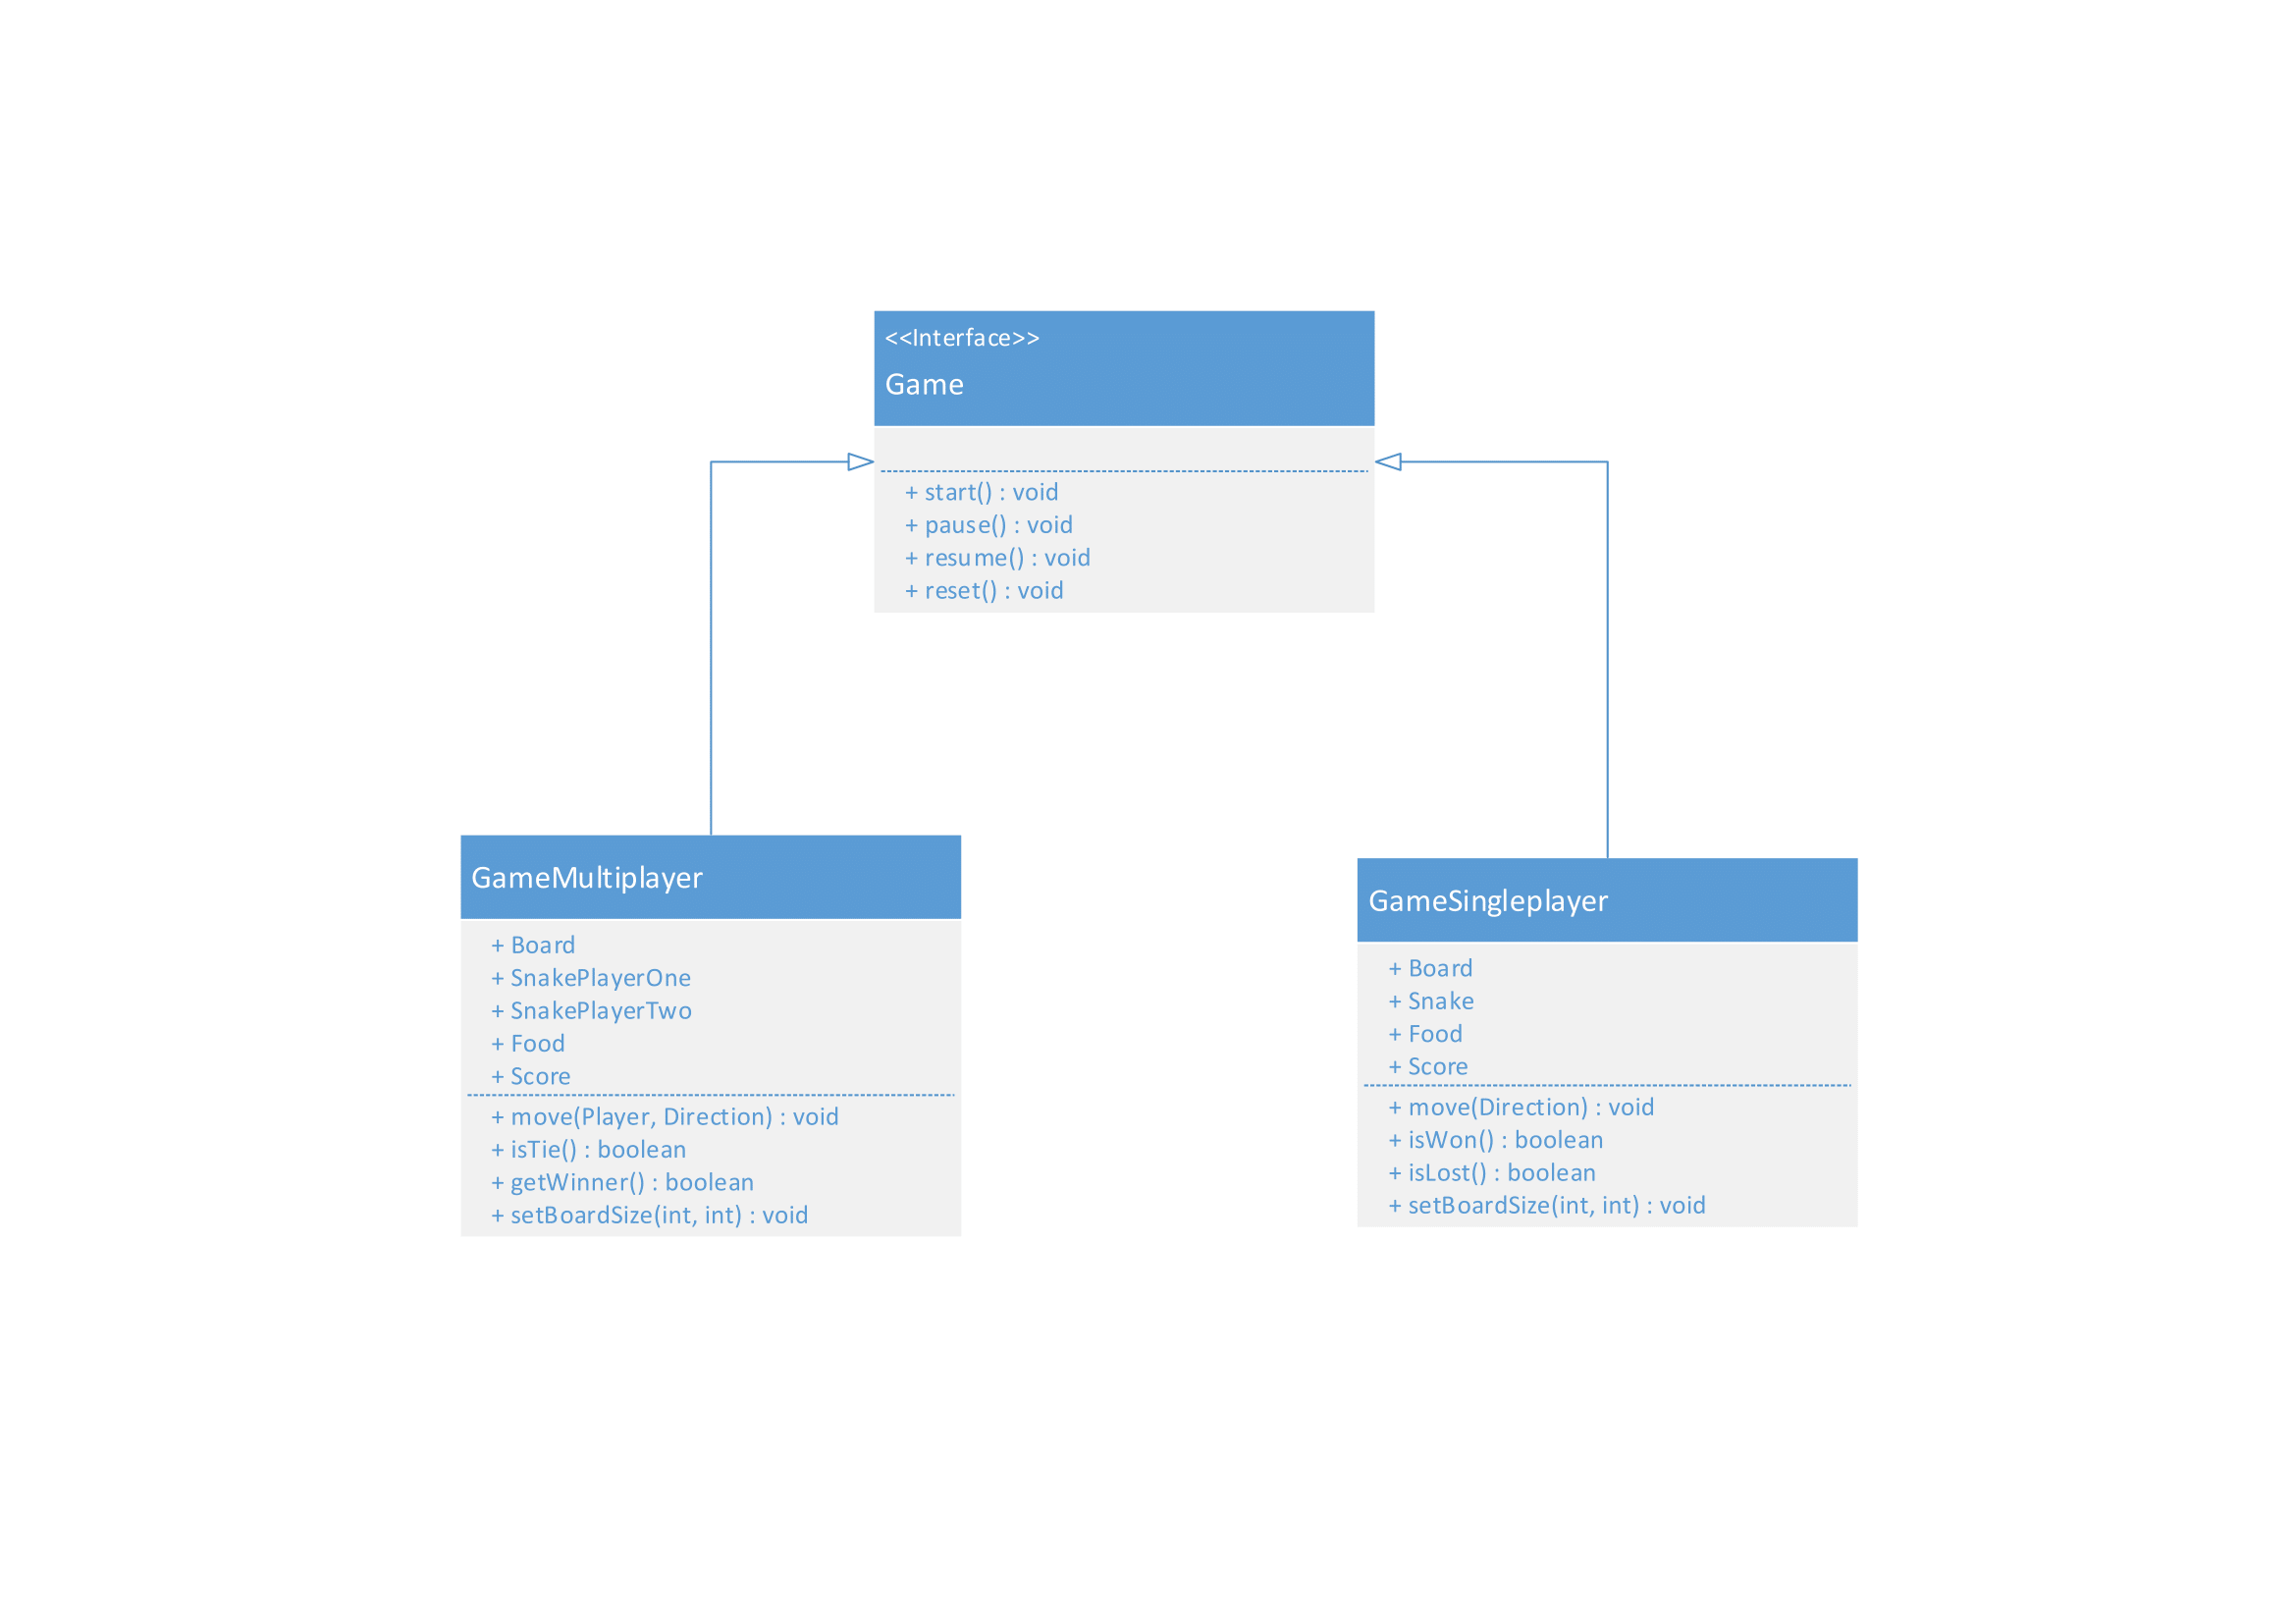
\includegraphics[width=1.0\textwidth]{advanceret/game-design.png}
	\hspace{0.1\textwidth}
	\figlab{game-design}
	\caption{\textit{Klassediagram over Game-klasserne.}}
\end{figure}

